%% Начало содержательной части.
\chapter{Глава 1. Обзор предметной области}

Пример ссылок на литературные источники: \cite{example-english, example-russian}.

\section{Таблицы}

В качестве примера таблицы приведена таблица~\ref{tab1}.

\begin{table}[!h]
\caption{Таблица умножения (фрагмент)}\label{tab1}
\centering
\begin{tabular}{|*{18}{c|}}\hline
-- & 1 & 2 & 3 & 4 & 5 & 6 & 7 & 8 & 9 & 10 & 11 & 12 & 13 & 14 & 15 & 16 & 17 \\\hline
1  & 1 & 2 & 3 & 4 & 5 & 6 & 7 & 8 & 9 & 10 & 11 & 12 & 13 & 14 & 15 & 16 & 17 \\\hline
2  & 2 & 4 & 6 & 8 & 10 & 12 & 14 & 16 & 18 & 20 & 22 & 24 & 26 & 28 & 30 & 32 & 34 \\\hline
3  & 3 & 6 & 9 & 12 & 15 & 18 & 21 & 24 & 27 & 30 & 33 & 36 & 39 & 42 & 45 & 48 & 51 \\\hline
4  & 4 & 8 & 12 & 16 & 20 & 24 & 28 & 32 & 36 & 40 & 44 & 48 & 52 & 56 & 60 & 64 & 68 \\\hline
\end{tabular}
\end{table}

Есть еще такое окружение \texttt{tabu}, его можно аккуратно растянуть на всю страницу.
Приведем пример (таблица~\ref{tab2}).

\begin{table}[!h]
\caption{Таблица умножения с помощью \texttt{tabu} (фрагмент)}\label{tab2}
\centering
\begin{tabu}{|*{18}{X[c]|}}\hline
-- & 1 & 2 & 3 & 4 & 5 & 6 & 7 & 8 & 9 & 10 & 11 & 12 & 13 & 14 & 15 & 16 & 17 \\\hline
1  & 1 & 2 & 3 & 4 & 5 & 6 & 7 & 8 & 9 & 10 & 11 & 12 & 13 & 14 & 15 & 16 & 17 \\\hline
2  & 2 & 4 & 6 & 8 & 10 & 12 & 14 & 16 & 18 & 20 & 22 & 24 & 26 & 28 & 30 & 32 & 34 \\\hline
3  & 3 & 6 & 9 & 12 & 15 & 18 & 21 & 24 & 27 & 30 & 33 & 36 & 39 & 42 & 45 & 48 & 51 \\\hline
4  & 4 & 8 & 12 & 16 & 20 & 24 & 28 & 32 & 36 & 40 & 44 & 48 & 52 & 56 & 60 & 64 & 68 \\\hline
\end{tabu}
\end{table}

\section{Рисунки}

Пример рисунка (c помощью \texttt{TikZ}) приведен на рисунке~\ref{fig1}. Под \texttt{pdflatex} можно также
использовать \texttt{*.jpg}, \texttt{*.png} и даже \texttt{*.pdf}, под \texttt{latex} можно использовать
Metapost. Последний можно использовать и под \texttt{pdflatex}, для чего в стилевике продекларированы
номера картинок от~1 до~20.

\begin{figure}[!h]
\caption{Пример рисунка}\label{fig1}
\centering
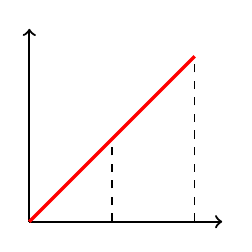
\begin{tikzpicture}[scale=0.7]
\draw[thick,->] (0,0)--(3.5,0);
\draw[thick,->] (0,0)--(0,3.5);
\draw[very thick, red] (0,0)--(3,3);
\draw[dashed] (3,0)--(3,3);
\draw[dashed] (1.5,0)--(1.5,1.5);
\end{tikzpicture}
\end{figure}

\section{Листинги}

В работах студентов кафедры <<Компьютерные технологии>> часто встречаются различные листинги. Листинги бывают
двух основных видов~--- исходный код и псевдокод. Первый оформляется с помощью окружения \texttt{lstlisting}
из пакета \texttt{listings}, который уже включается в стилевике и немного настроен. Пример Hello World на Java
приведен на листинге~\ref{lst1}.

\begin{lstlisting}[float=!h,caption={Пример исходного кода на Java},label={lst1}]
public class HelloWorld {
	public static void main(String[] args) {
		System.out.println("Hello, world!");
	}
}
\end{lstlisting}

Псевдокод можно оформлять с помощью разных пакетов. В данном стилевике включается пакет \texttt{algorithmicx}.
Сам по себе он не генерирует флоатов, поэтому для них используется пакет \texttt{algorithm}.
Пример их совместного использования приведен на листинге~\ref{lst2}. Обратите внимание, что флоаты разные, а 
нумерация~--- общая!

\begin{algorithm}[!h]
\caption{Пример псевдокода}\label{lst2}
\begin{algorithmic}
	\Function{IsPrime}{$N$}
		\For{$t \gets [2; \lfloor\sqrt{N}\rfloor]$}
			\If{$N \bmod t = 0$}
				\State\Return \textsc{false}
			\EndIf
		\EndFor
		\State\Return \textsc{true}
	\EndFunction
\end{algorithmic}
\end{algorithm}

Наконец, листинги из \texttt{listings} тоже можно подвешивать с помощью \texttt{algorithm},
пример на листинге~\ref{lst3}.

\begin{algorithm}[!h]
\caption{Исходный код и флоат \texttt{algorithm}}\label{lst3}
\begin{lstlisting}
public class HelloWorld {
	public static void main(String[] args) {
		System.out.println("Hello, world!");
	}
}
\end{lstlisting}
\end{algorithm}
